\documentclass[beamer, crop, multi = true, tikz]{standalone}
\usepackage{booktabs}
\usepackage{pgfplots}
\pgfplotsset{compat=newest}
\usepgfplotslibrary{groupplots}
\usepgfplotslibrary{polar}
\usepgfplotslibrary{smithchart}
\usepgfplotslibrary{statistics}
\usepgfplotslibrary{dateplot}
\usepgfplotslibrary{ternary}
\usetikzlibrary{arrows.meta}
\usetikzlibrary{backgrounds}
\usepgfplotslibrary{patchplots}
\usepgfplotslibrary{fillbetween}

\begin{document}
\begin{standaloneframe}[fragile]
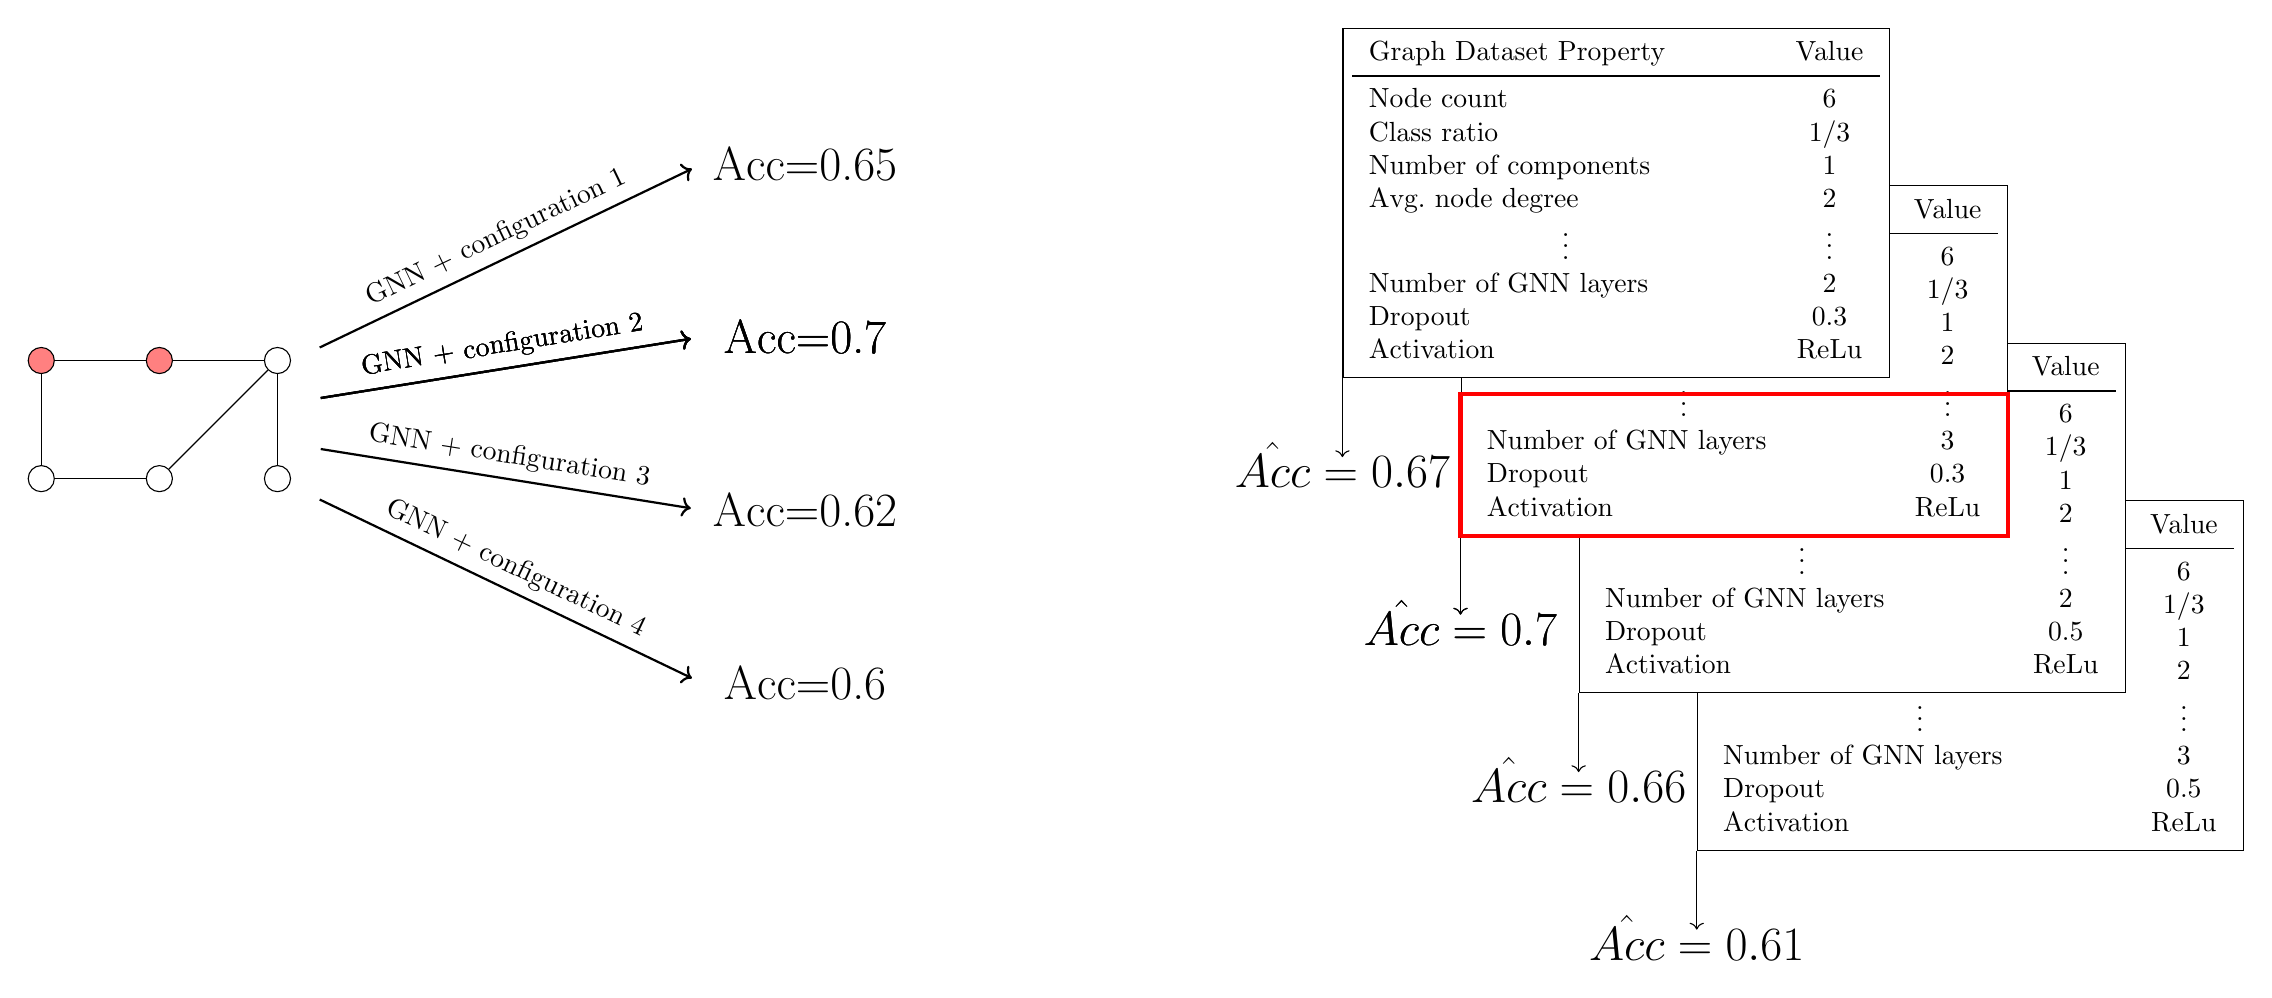
\begin{tikzpicture}
\def\dist{1.5cm}
\tikzset{node distance=\dist, minimum size=1ex}

	\tikzset{classA/.style={circle, draw=black, fill=blue!20!yellow}}
	\tikzset{classB/.style={circle, draw=black, fill=blue!20}}
	\tikzset{classC/.style={circle, draw=black, fill=yellow!20!red}}
	\tikzset{class1/.style={circle, draw=black, fill=red!50}}
	\tikzset{class0/.style={circle, draw=black, fill=white}}
	\tikzset{desc/.style={rectangle, anchor=west, text width=2.5cm,minimum height=1cm,minimum width=2.8cm, rounded corners=1ex, align=center}}

	\newcommand{\drawgraph}[9]{%
\begin{scope}[xshift=#1, yshift=#2]
\node[#3] (#9A1) {};
\node[#4, right of=#9A1] (#9A2) {};
\node[#5, below of=#9A1] (#9B1) {};
\node[#6, right of=#9A2] (#9B2) {};
\node[#7, below of=#9A2] (#9C1) {};
\node[#8, below of=#9B2] (#9C2) {};
\draw [-] (#9A1) -- (#9A2);
\draw [-] (#9A1) -- (#9B1);
\draw [-] (#9B1) -- (#9C1);
\draw [-] (#9C1) -- (#9B2);
\draw [-] (#9B2) -- (#9C2);
\draw [-] (#9A2) -- (#9B2);
\end{scope}
	}

\drawgraph{-12cm}{7.5cm}{class1}{class1}{class0}{class0}{class0}{class0}{task1}

%\node[fill=white, draw] (r4) at (8, 9.5) {
%	 \begin{tabular}{p{5cm}c}
%		 Graph Dataset Property & Value  \\
%		 \midrule
%		 Node count				& 6		 \\
%		 Class ratio			& 1/3	 \\
%		 Number of components	& 1		 \\
%		 Avg. node degree		& 2    \\
%		 \centerline{\vdots}	& \vdots \\
%	 \end{tabular}};

\uncover<1->{%
\draw[->, thick, shorten >=1ex, shorten <=1ex] (-8.6,7.6) -- +(5,2.4) node [pos=0.5, above, sloped] {GNN + configuration 1} node [font=\LARGE, pos=1, xshift=1.3cm] {Acc=0.65};

\draw[->, thick, shorten >=1ex, shorten <=1ex] (-8.6,7) -- +(5,0.8) node [pos=0.5, above, sloped] {GNN + configuration 2}  node [font=\LARGE, pos=1, xshift=1.3cm] {Acc=0.7};

\draw[->, thick, shorten >=1ex, shorten <=1ex] (-8.6,6.4) -- +(5,-0.8) node [pos=0.5, above, sloped] {GNN + configuration 3}  node [font=\LARGE, pos=1, xshift=1.3cm] {Acc=0.62};

\draw[->, thick, shorten >=1ex, shorten <=1ex] (-8.6,5.8) -- +(5,-2.4) node [pos=0.5, above, sloped] {GNN + configuration 4}  node [font=\LARGE, pos=1, xshift=1.3cm] {Acc=0.6};


\node[fill=white, draw] (r4) at (12.5, 3.5) {%
	\begin{tabular}{p{5cm}c}
		Graph Dataset Property & Value	\\
		\midrule
		Node count			   & 6		\\
		Class ratio			   & 1/3	\\
		Number of components   & 1		\\
		Avg.\ node degree		& 2    \\
		\centerline{\vdots}    & \vdots \\
		Number of GNN layers   & 3		\\
		Dropout				   & 0.5	\\
		Activation			   & ReLu	\\
	\end{tabular}
};

\node[fill=white, draw] (r3) at (11, 5.5) {%
	\begin{tabular}{p{5cm}c}
		Graph Dataset Property & Value	\\
		\midrule
		Node count			   & 6		\\
		Class ratio			   & 1/3	\\
		Number of components   & 1		\\
		Avg.\ node degree		& 2    \\
		\centerline{\vdots}    & \vdots \\
		Number of GNN layers   & 2		\\
		Dropout				   & 0.5	\\
		Activation			   & ReLu	\\
	\end{tabular}
};


\node[fill=white, draw] (r2) at (9.5, 7.5) {%
	\begin{tabular}{p{5cm}c}
		Graph Dataset Property & Value	\\
		\midrule
		Node count			   & 6		\\
		Class ratio			   & 1/3	\\
		Number of components   & 1		\\
		Avg.\ node degree		& 2    \\
		\centerline{\vdots}    & \vdots \\
		Number of GNN layers   & 3		\\
		Dropout				   & 0.3	\\
		Activation			   & ReLu	\\
	\end{tabular}
};


\node[fill=white, draw] (r1) at (8, 9.5) {%
	\begin{tabular}{p{5cm}c}
		Graph Dataset Property & Value	\\
		\midrule
		Node count			   & 6		\\
		Class ratio			   & 1/3	\\
		Number of components   & 1		\\
		Avg.\ node degree		& 2    \\
		\centerline{\vdots}    & \vdots \\
		Number of GNN layers   & 2		\\
		Dropout				   & 0.3	\\
		Activation			   & ReLu	\\
	\end{tabular}
};


\draw[->] (r1.south west) -- node[font=\LARGE,pos=1.1] {$\hat{Acc}=0.67$} ([yshift=-1cm] r1.south west);
\draw[->] (r2.south west) -- node[font=\LARGE,pos=1.1] (mmax) {$\hat{Acc}=0.7$} ([yshift=-1cm] r2.south west);
\draw[->] (r3.south west) -- node[font=\LARGE,pos=1.1] {$\hat{Acc}=0.66$} ([yshift=-1cm] r3.south west);
\draw[->] (r4.south west) -- node[font=\LARGE,pos=1.1] {$\hat{Acc}=0.61$} ([yshift=-1cm] r4.south west);
}
\uncover<2->{%
%\draw[color=red, ultra ]  (mmax.center) circle (1.3cm);
\draw[->] (r2.south west) -- node[font=\LARGE,pos=1.1] (mmax) {\alert{$\hat{Acc}=0.7$}}([yshift=-1cm] r2.south west);

\draw[->, thick, shorten >=1ex, shorten <=1ex] (-8.6,7) -- +(5,0.8) node [pos=0.5, above, sloped] {GNN + configuration 2}  node [font=\LARGE, pos=1, xshift=1.3cm] {\alert{Acc=0.7}};
}
\uncover<3->{%
\draw[color=red, ultra thick]  (r2.south west) rectangle ([yshift=1.8cm] r2.south east);

\draw[->, thick, shorten >=1ex, shorten <=1ex] (-8.6,7) -- +(5,0.8) node [pos=0.5, above, sloped] {GNN + \alert{configuration 2}}  node [font=\LARGE, pos=1, xshift=1.3cm] {\alert{Acc=0.7}};
}
\end{tikzpicture}
\end{standaloneframe}
\end{document}
